%% Supplementary Information for the Nature Communications build. Written 2026-09-11.
%%
%% Numbering follows the journal: Supplementary Note N, Supplementary Table N, Supplementary Figure N,
%% each cited from the main text at the sentence whose claim it supports. Every number here is one a
%% committed result file states, and paper/check_numbers.py binds them.
%%
%% EMBARGO. Nothing from the embargoed external cohort may appear here until its permission file
%% records permission.
%%
%% Figures are NOT copied into this directory. \graphicspath points at where they are built.

\documentclass[11pt]{article}
\usepackage[utf8]{inputenc}
\usepackage[T1]{fontenc}
\usepackage[a4paper, margin=2.4cm]{geometry}
\usepackage{graphicx}
\graphicspath{{../figures/}}
\usepackage{booktabs}
\usepackage{longtable}
\usepackage{array}
\usepackage{amsmath}
\usepackage[numbers,sort&compress]{natbib}
\usepackage[hidelinks]{hyperref}
\usepackage{xcolor}

\newcommand{\TODO}[1]{\textcolor{red}{[TODO: #1]}}
\renewcommand{\tablename}{Supplementary Table}
\renewcommand{\figurename}{Supplementary Figure}
\newcounter{snote}
\newcommand{\snote}[1]{\refstepcounter{snote}\section*{Supplementary Note~\thesnote. #1}%
  \addcontentsline{toc}{section}{Supplementary Note~\thesnote. #1}}

\renewcommand{\topfraction}{0.95}
\renewcommand{\bottomfraction}{0.7}
\renewcommand{\textfraction}{0.07}
\renewcommand{\floatpagefraction}{0.75}

\title{Supplementary Information\\[0.4em]
\large Parameter-free fusion of histology, transcriptome and stage predicts bladder cancer survival
against a correctly specified clinical reference}
\author{Guanxing Chen}
\date{}

\begin{document}
\maketitle
\tableofcontents
\newpage

%% ============================================================================ NOTE 1
\snote{The clinical-baseline census, and why grade cannot separate patients}
\label{note:census}

The main text's claim about the benchmark's clinical reference is a claim about other papers, so it
is given here one paper at a time (Supplementary Table~\ref{tab:census}). A row reads
``verified'' only where the covariate sentence was read in the paper itself. Where the text could
not be read, the row says so and is not filled in from the pattern of the others.

\begin{table}[h]
\centering
{\small
\begin{tabular}{llll}
\toprule
paper & venue & clinical baseline & stage \\
\midrule
PORPOISE~\citep{chen2022porpoise} & Cancer Cell 2022 & age, gender, tumour grade & not used \\
SurvPath~\citep{jaume2024survpath} & CVPR 2024 & age, sex, grade & not used \\
PIBD~\citep{zhang2024pibd} & ICLR 2024 & \emph{reports no clinical baseline} & n/a \\
MOTCat~\citep{xu2023motcat} & ICCV 2023 & \emph{reports no clinical baseline} & n/a \\
MMP~\citep{song2024mmp} & ICML 2024 & age, sex, cancer grade & not used \\
DIMAF~\citep{eijpe2025dimaf} & MICCAI 2025 & grade, age, sex & not used \\
OTSurv~\citep{ren2025otsurv} & MICCAI 2025 & \emph{reports no clinical baseline} & n/a \\
DSCASurv~\citep{song2025dscasurv} & Brief.\ Bioinform.\ 2025 & \emph{reports no clinical baseline} & n/a \\
MCAT~\citep{chen2021mcat} & ICCV 2021 & \emph{not verified} & n/a \\
MOAD-FNet~\citep{moadfnet2024} & arXiv 2024 & \emph{not verified} & n/a \\
APL~\citep{apl2025} & arXiv 2025 & \emph{not verified} & n/a \\
\bottomrule
\end{tabular}}
\caption{Every method paper associated with the benchmark, and what it compares against. Of the
eight whose text could be read, four report a clinical-variable baseline and all four build it
from grade. None uses pathologic stage, and four report no clinical baseline at all. Three could
not be verified and are marked as such. The bladder values the four report are 0.519 (DIMAF) and
0.570 (SurvPath and MMP, age, sex and grade).}
\label{tab:census}
\end{table}

\noindent The covariate statements behind the four verified rows, quoted from each paper:
\begin{itemize}
  \item \textbf{PORPOISE}: Cox models ``using age, gender, and tumor grade covariates as
    baselines'' (main text, referring to its Table S4).
  \item \textbf{SurvPath}: ``Age, Sex, Grade'' (Supplementary Table 3).
  \item \textbf{MMP}: ``age, sex, and cancer grade as reported in the TCGA cohort'' (Table 1
    caption).
  \item \textbf{DIMAF}: ``a clinical baseline using grade, age, and sex'' (Table 1, clinical row).
\end{itemize}

\noindent Half of the papers that could be read compare against no clinical variable at all, only
against other deep-learning models. On this benchmark the comparison with the clinic is therefore
either made against a covariate that cannot separate these patients, or not made.

\paragraph{Why grade cannot work in this disease.} Supplementary Table~\ref{tab:entropy} sets the
two covariates side by side in each of the five studies the benchmark covers. Bladder is the extreme
case. Muscle-invasive urothelial carcinoma is almost uniformly high grade, and in this cohort grade
takes two levels with 94.4\% of patients in one of them. A covariate that does not distinguish the
patients cannot separate them, whatever model is fitted on top of it.

\begin{table}[h]
\centering
{\small
\setlength{\tabcolsep}{4pt}
\begin{tabular}{lcccccccc}
\toprule
 & & \multicolumn{3}{c}{grade} & \multicolumn{3}{c}{stage} & \\
\cmidrule(lr){3-5}\cmidrule(lr){6-8}
study & $n$ & levels & modal & entropy & levels & modal & entropy & stage $-$ grade \\
\midrule
bladder & 359 & 2 & 94.4\% & 0.311 & 5 & 50.6\% & 0.665 & $+0.0560$ \\
breast & 871 & \multicolumn{3}{c}{no usable grade in the released file} & 5 & 60.3\% & 0.631 & $+0.0858$ \\
colorectal & 298 & \multicolumn{3}{c}{no usable grade in the released file} & 5 & 68.7\% & 0.572 & $+0.2208$ \\
head and neck & 394 & 5 & 59.7\% & 0.643 & 5 & 37.5\% & 0.884 & $+0.0423$ \\
stomach & 319 & 4 & 58.9\% & 0.623 & 4 & 47.3\% & 0.835 & $+0.0461$ \\
\bottomrule
\end{tabular}}
\caption{Level composition and normalised Shannon entropy of grade and stage in the five studies,
and the concordance gained by swapping one for the other. Every row uses the clinical files released
with the benchmark, the only clinical source common to all five studies. The bladder result in the
main text (0.6638 against 0.5666) takes every column from the incumbent's own split files instead,
which makes it a statement about the incumbent's baseline. On bladder, this table's source gives
$+0.0560$. Two studies ship no usable grade, so there the ``grade'' arm is age and sex alone and the
comparison shows stage improving that baseline. They are marked rather than dropped.}
\label{tab:entropy}
\end{table}

%% ============================================================================ NOTE 2
\snote{The frozen protocol, its amendment, the falsifiers and the selection correction}
\label{note:protocol}

\paragraph{The protocol.} The protocol fixed the arm, the estimator, the penalty grid, the
combination rule, the comparator set, the seeds and the decision rule. It was written after the
development campaign and the leakage falsifiers, and before the confirmatory run. Its rule was:
primary above $0.679 + 0.0239$, and a standard deviation across seeds of at most 0.0145, where
0.0239 is $\sigma\sqrt{2\ln N}$ with $\sigma = 0.0073$ and the $N = 211$ candidates the development
ledger held when the protocol was written. The second condition is a stability requirement and it
holds (0.0048). The first is mis-specified, as the last paragraph of this note shows.

\paragraph{Amendment A1, and its two opposite effects.} A cached clinical query had taken the first
of several diagnosis records per patient, and 61 of 359 patients changed once the correct record was
chosen. The tell was present before the check: stage IIA, IIB and IIC appear in that record and are
not AJCC bladder stages. Fixing the record is worth $+0.0050$ on ModRank. Rebuilding the block from
the incumbent's own released columns also removes the T, N and M categories the cached query had
supplied, which is worth $-0.0110$. Net, the reported primary fell from 0.7260 to 0.7212, a move of
$-0.0048$, and the lower value is the one reported.

\paragraph{The falsifiers.} Five leakage falsifiers ran before the confirmatory run: fold integrity,
a mutation test of the standardisation boundary, a per-fold planted label, row permutation and
outcome provenance. Two were built to reject and did. The planted-label falsifier was wrong on its
first construction. One column built for the whole cohort placed the outcome ordering on every
training row as well as every validation row, because each patient sits in exactly one validation
fold, and it reported a spurious 0.8715. Rebuilt per fold, it moves the score by $-0.0006$.

\paragraph{The development campaign.} The campaign scored 269 candidate arms in a ledger generated
from the runs' own output. The protocol recorded 211 because that is what the ledger held when it was
written. Two further sub-experiments (58 rows) were scored afterwards and before the confirmatory
run. Not all 269 are candidates the frozen arm competed against: 26 are subgroup slices scored on part
of the cohort, 18 are in-sample oracles, 14 are permuted or null controls and 5 are cross-cohort
transfer probes. That leaves 206 full-cohort out-of-fold candidates. Among them the frozen
configuration is rank 11 counting every tie against it. Eight configurations score strictly above:
two are another TCGA study, three are components rejected on their own pre-registered controls, and
the rest are the declared transcriptomic sensitivity. The remaining two places are the frozen
construction's own duplicates, logged three times by three sub-experiments. Seven components were
designed, each with a falsifier and, where one could be built, a matched control. None cleared the
0.0145 bar (Supplementary Table~\ref{tab:components} and Supplementary Figure~\ref{fig:campaign}).

\begin{table}[h]
\centering
{\small
\begin{tabular}{cllccl}
\toprule
 & component & predicted & observed & control & status \\
\midrule
C1 & pan-cancer survival subspace prior & $+0.0300$ & $-0.0042$ & $-0.0141$ & void \\
C1$'$ & the same direction, zero-shot & $+0.0250$ & $+0.0033$ & $-0.0311$ & void \\
C2 & bagged ridge & $+0.0400$ & $-0.0561$ & n/a & graded \\
C4 & dense regularisation path & $+0.0200$ & $-0.0042$ & n/a & void \\
C5 & gated fusion on clinical risk & $+0.0200$ & $+0.0046$ & $+0.0055$ & void \\
C6 & inner-CV skill weighting & $+0.0200$ & $+0.0105$ & n/a & void \\
C7 & stratified partial likelihood & $+0.0300$ & $-0.0199$ & $-0.0095$ & graded \\
\bottomrule
\end{tabular}}
\caption{The seven falsified components. Every predicted value was fixed before the run. The bar is
0.0145, twice the measured split-reseed standard deviation. None cleared it. Status is as recorded
in the development ledger, where void marks a result that its own control leaves unreadable and
graded marks a readable result that fails the bar.}
\label{tab:components}
\end{table}

\begin{figure}[h]
\centering
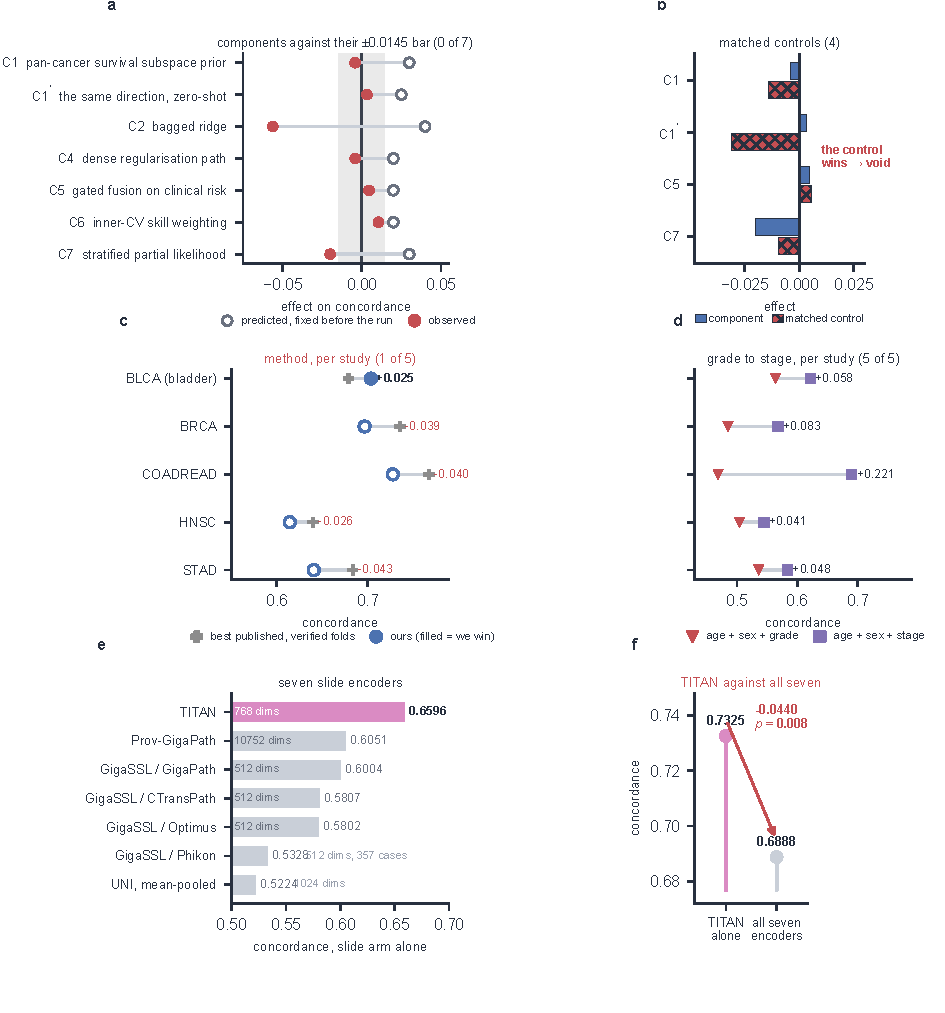
\includegraphics[width=\textwidth]{figS1_campaign.pdf}
\caption{\textbf{The development campaign, its generalisation and its representations.}
\textbf{a},~What each of the seven components was predicted to be worth, fixed before the run,
against what it was worth. The shaded band is the $\pm0.0145$ bar. \textbf{b},~The four components
that carry a matched control. C5's control beats it, which is what a void looks like.
\textbf{c},~ModRank against the best published entry with verified folds, per study. Bladder wins and
four of five lose. \textbf{d},~The one-column swap in the same five studies, five of five.
\textbf{e},~Seven slide encoders scored as single arms on identical patients and folds.
\textbf{f},~The seven-encoder pool against TITAN alone, paired on patients.}
\label{fig:campaign}
\end{figure}

\paragraph{The selection correction was mis-specified.} A correction for taking the best of $N$
candidates, of the form $\sigma\sqrt{2\ln N}$, needs $\sigma$ to be the spread of one candidate's
own absolute score when no signal is present. The protocol substituted the spread of a paired difference between two arms
(0.0073), which is the quantity the noise floor measures and a different one. We measured the right
quantity directly. Across 200 permutations of the survival outcome, with folds, features and the
estimator untouched, the 14 fusion candidates of the final family score a mean of 0.5011 and a
standard deviation of 0.0397. The Gaussian bar with that $\sigma$ at $N = 206$ is 0.8087. The
empirical alternative needs no independence assumption, because the permuted candidates are
correlated in exactly the way the real search was. The 95th percentile of the null maximum over the
family is 0.5926, an inflation of 0.0926 above chance, which sets the bar at 0.7716. The primary
(0.7212) clears neither. The paper therefore makes no selection-corrected claim. Its claim about the
benchmark is the one the data support: the highest concordance reported on these folds, by point
estimate, with the paired comparisons against the two competitors that could be rerun reported as
not significant.

%% ============================================================================ NOTE 3
\snote{What each arm carries}
\label{note:arms}

\paragraph{Every arm at every seed.} The primary is a mean over five inner-cross-validation seeds, so
the individual values are given (Supplementary Table~\ref{tab:perseed}). Three quantities that the
main text keeps distinct can be reconstructed from them: the primary (0.7212), the seed-0 value
(0.7225) and the concordance of the seed-averaged score vector (0.7237), which is the one every
paired comparison uses.

\begin{table}[h]
\centering
{\small
\begin{tabular}{ccccc}
\toprule
seed & ModRank & slide & transcriptome & clinical \\
\midrule
0 & 0.7225 & 0.6596 & 0.6510 & 0.6638 \\
1 & 0.7248 & 0.6515 & 0.6733 & 0.6657 \\
2 & 0.7129 & 0.6550 & 0.6470 & 0.6638 \\
3 & 0.7243 & 0.6553 & 0.6664 & 0.6644 \\
4 & 0.7216 & 0.6472 & 0.6681 & 0.6666 \\
\midrule
mean & 0.7212 & & & \\
standard deviation & 0.0048 & & & \\
\bottomrule
\end{tabular}}
\caption{Concordance of each arm at each inner-cross-validation seed on the released folds.}
\label{tab:perseed}
\end{table}

\paragraph{Where the slide separates patients the report cannot.} Supplementary
Table~\ref{tab:ties} restricts the comparable pairs to those the clinical model places close
together, at four widths. As the restriction tightens, the clinical arm falls from 0.6638 to
0.4959, which is chance by construction, while the slide arm stays between 0.6220 and 0.6368. A second restriction asks the same question
of the transcriptome. On the 9,688 pairs whose transcriptome-arm scores are closest (the 40\% with
the smallest gap) the slide arm reaches 0.6396 while the transcriptome arm is at 0.5604. On the
3,893 pairs that are that close on the transcriptome arm and also within the closest 40\% on the
clinical model, the slide arm reaches 0.6212, against 0.5543 and 0.5634 for the two arms that define
the restriction. Read with ``stage'' as the same stage group rather than the clinical model, the
restriction keeps 3,183 pairs and the slide arm reaches 0.6030. These are statements about two
particular scores. They do not show that no transcriptomic model could recover the same information.

\begin{table}[h]
\centering
{\small
\begin{tabular}{lcccc}
\toprule
restriction & pairs & clinical & slide & incumbent \\
\midrule
all comparable pairs & 24,219 & 0.6638 & 0.6596 & 0.6118 \\
closest 40\% on the clinical model & 9,695 & 0.5661 & 0.6368 & 0.5873 \\
closest 20\% & 4,844 & 0.5319 & 0.6361 & 0.5969 \\
closest 10\% & 2,423 & 0.5107 & 0.6271 & 0.5999 \\
closest 5\% & 1,213 & 0.4959 & 0.6220 & 0.5952 \\
\bottomrule
\end{tabular}}
\caption{Concordance on comparable pairs restricted by how close the clinical model places the two
patients, at seed 0 with the amended clinical block. The incumbent column is SurvPath's own
out-of-fold risk.}
\label{tab:ties}
\end{table}

\paragraph{What the two molecular-facing arms track.} Against eight standard axes of
muscle-invasive bladder cancer biology, the transcriptome arm reads molecular class: its Spearman
correlation is 0.3595 with the basal axis, $-0.372$ with the luminal axis and 0.3672 with the
epithelial--mesenchymal axis, all after Benjamini--Hochberg correction. The slide arm's correlation
with the basal axis is 0.0438 and does not survive correction. Its largest axis correlation is with
the FGFR3 axis ($-0.2245$), which carries no univariate prognostic signal in this cohort. Over all
275 pathway scores, 59 reach $q<0.05$ against the slide arm, and the two strongest are metabolic:
fatty acids ($-0.287$) and arachidonate production from diacylglycerol (0.278). These are
associations between an out-of-fold score and a pathway mean over 275 correlated tests. They say
what the score varies with, not that the model reads that pathway. No single pathway clears
Benjamini--Hochberg $q<0.10$ as a univariate predictor of disease-specific survival
(Supplementary Figure~\ref{fig:landscape}), so whatever the transcriptome arm contributes, it does
not contribute through one programme.

\paragraph{The two modalities are informative in different tumours.} The released files carry no
subtype call, so the cohort was split at the median of the basal-minus-luminal signature
difference. The axis is itself prognostic (log-rank $p=0.0012$). Inside the two halves the slide and
clinical arms exchange places, and ModRank moves far less than either
(Supplementary Table~\ref{tab:subtype} and Supplementary Figure~\ref{fig:biology}).

\begin{table}[h]
\centering
{\small
\begin{tabular}{lccccc}
\toprule
half & $n$ / events & clinical & slide & transcriptome & ModRank \\
\midrule
basal-leaning & 179 / 71 & 0.6472 & 0.6693 & 0.6226 & 0.7109 \\
luminal-leaning & 180 / 42 & 0.7005 & 0.6197 & 0.6218 & 0.6997 \\
\bottomrule
\end{tabular}}
\caption{Concordance within the two halves of the basal-minus-luminal signature axis, split at its
median.}
\label{tab:subtype}
\end{table}

\begin{figure}[p]
\centering
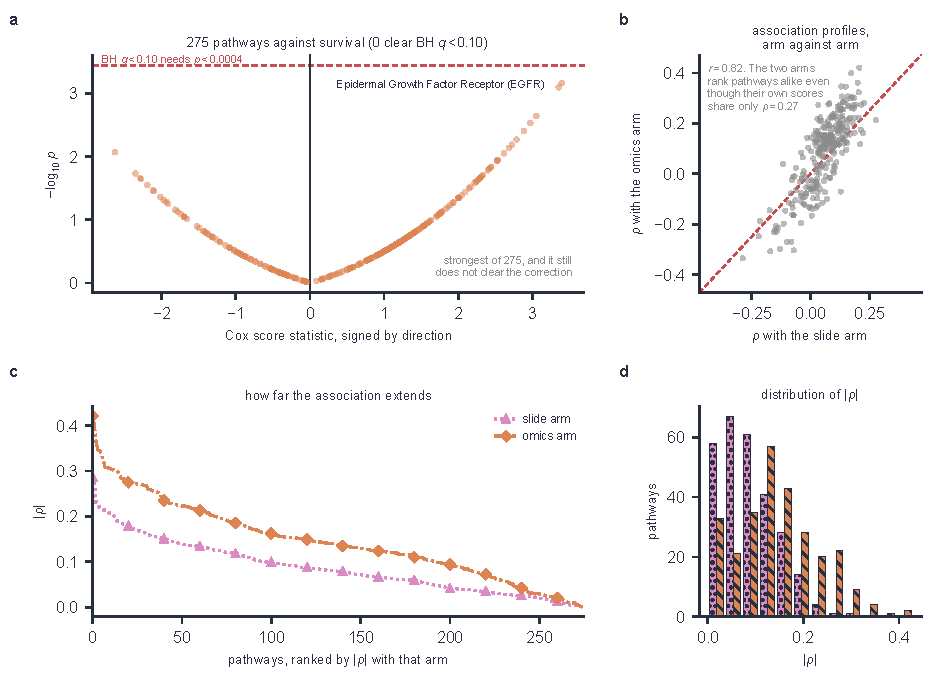
\includegraphics[width=\textwidth]{figS4_pathway_landscape.pdf}
\caption{\textbf{All 275 pathways.} \textbf{a},~Univariate Cox score statistic against
$-\log_{10} p$, signed by whether the pathway scores above or below chance as a raw risk score. The
dashed line is the smallest $p$ that would clear Benjamini--Hochberg at $q<0.10$, and no pathway
reaches it. \textbf{b},~Each pathway's Spearman correlation with the slide arm against its
correlation with the transcriptome arm. \textbf{c},~\textbf{d},~How far the association extends,
ranked and binned.}
\label{fig:landscape}
\end{figure}

\begin{figure}[p]
\centering
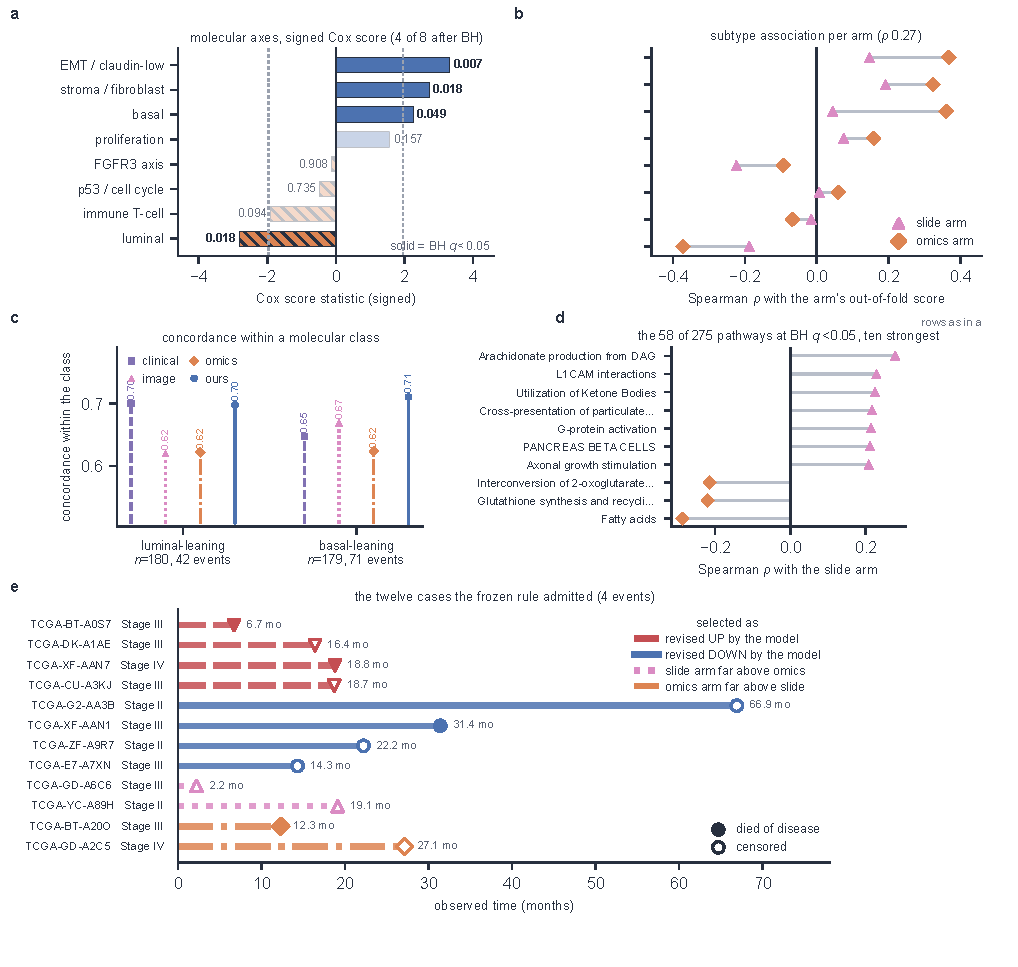
\includegraphics[width=\textwidth]{fig5_biology.pdf}
\caption{\textbf{What the two molecular-facing arms read.} Descriptive throughout.
\textbf{a},~Four of the eight axes are prognostic after Benjamini--Hochberg correction.
\textbf{b},~The transcriptome arm reads molecular class and the slide arm does not.
\textbf{c},~Concordance inside each half of the basal-minus-luminal axis. \textbf{d},~The ten
strongest of the slide arm's 275 pathway associations. \textbf{e},~The twelve patients of the
second pre-specified case series.}
\label{fig:biology}
\end{figure}

\begin{figure}[p]
\centering
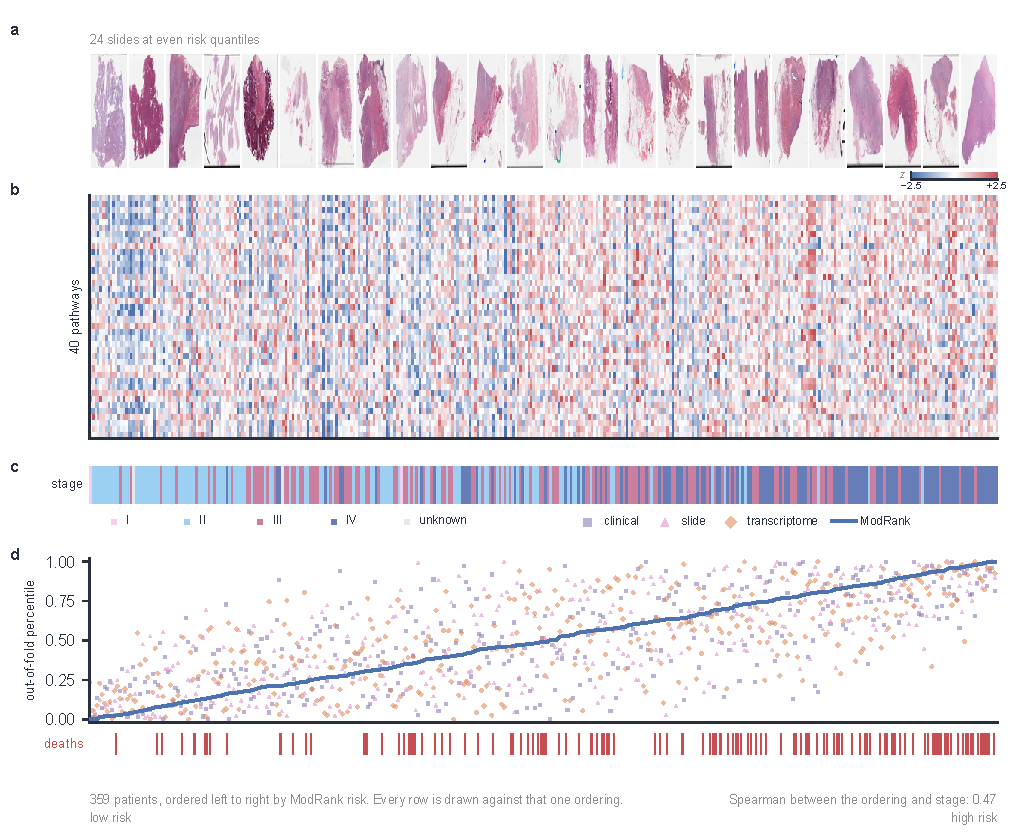
\includegraphics[width=\textwidth]{fig5_cohort_modalities.pdf}
\caption{\textbf{All three modalities across the cohort, on one patient axis.} All 359 patients,
ordered by ModRank risk, with every row drawn against that ordering. \textbf{a},~Twenty-four
diagnostic slides sampled at even risk quantiles, at matched physical resolution. \textbf{b},~The
forty pathways with the strongest univariate association, standardised across the cohort, one column
per patient. The arm itself reads all 275. \textbf{c},~Pathologic stage. Higher stages are enriched
to the right, but the row is not sorted, and the rank correlation between the ordering and stage is
printed in the panel. \textbf{d},~The three arm percentiles against the same ordering, with the
ModRank curve through them and a rug of the 113 deaths.}
\label{fig:cohort}
\end{figure}

\begin{figure}[p]
\centering
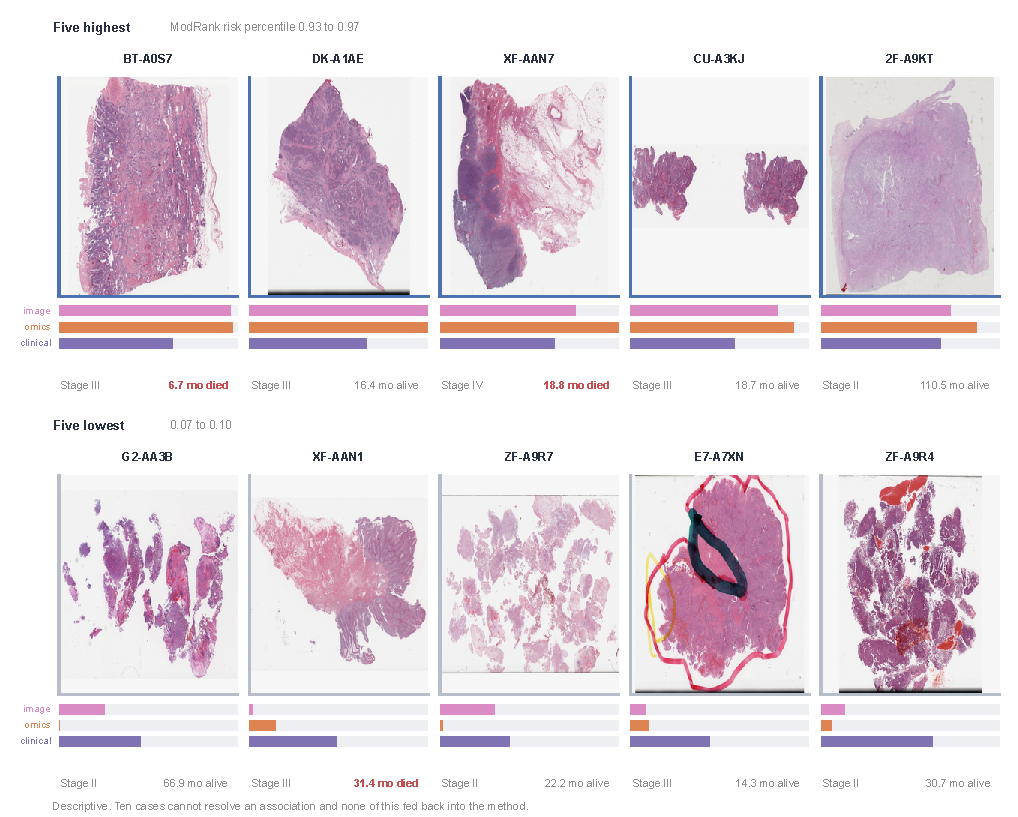
\includegraphics[width=\textwidth]{fig4_case_array.pdf}
\caption{\textbf{The ten patients of the first pre-specified case series, with their histology.}
Within the middle tertile of the clinical model's risk, the five patients ModRank scores highest
(above) and the five it scores lowest (below), with one diagnostic slide per patient at matched
physical resolution. Under each slide the three modality percentiles are drawn as a stack. The
series is reported whole, including the patients the model gets wrong: TCGA-XF-AAN1 is among the
five lowest and died at 31.4 months, and TCGA-2F-A9KT is among the five highest and was alive at
110.5 months. Ten patients cannot resolve an association, and the selection rule was fixed before
any output was inspected.}
\label{fig:cases}
\end{figure}

%% ============================================================================ NOTE 4
\snote{The external cohorts}
\label{note:geo}

\paragraph{Selection.} Public bladder series in the Gene Expression Omnibus were admitted only on a
counted yes: expression, stage, grade, age, sex and a timed disease-specific outcome recorded for the
same samples. The count was made from the series' characteristic fields before any outcome was
analysed. Three cohorts were admitted: GSE31684 (93 patients treated by radical cystectomy, Affymetrix
GPL570)~\citep{riester2012combination}, GSE32894 (the Lund cohort of non-muscle-invasive and
muscle-invasive tumours, Illumina GPL6947)~\citep{sjodahl2012molecular} and GSE48075 (GPL6947, no
grade field, so used for the combination rule only)~\citep{choi2014identification}. Three further
series were excluded: one repeats the samples of GSE48075, one holds cell lines, and one mixes
patients given neoadjuvant chemotherapy into the cohort and records no grade.

\paragraph{Protocol.} The protocol was frozen before any outcome of these cohorts was analysed. It
fixes the endpoints (death from bladder cancer), the clinical blocks, probe-to-gene mapping from the
platform annotation, the same pathway definitions as the benchmark (keeping groups with at least
three genes present), five repeats of stratified five-fold cross-validation, paired comparisons on
repeat-averaged scores with 6,000 patient resamples and Holm correction within each cohort, and a
noise floor from 24 re-partitions. The recipe is refitted inside each cohort. No coefficient fitted
on the development cohort is transferred across platforms. The protocol also recorded, before the
run, that the inflation $D$ should be smaller in the Lund cohort, where grade varies, than in the
cystectomy cohort. It was larger, and that prediction is reported as wrong.

\begin{table}[h]
\centering
{\small
\setlength{\tabcolsep}{4pt}
\begin{tabular}{lccc}
\toprule
 & GSE31684 & GSE32894 & GSE48075 \\
\midrule
setting & cystectomy & mixed & mixed \\
patients / deaths from the disease & 93 / 38 & 224 / 25 & 73 / 35 \\
pathway groups kept & 274 & 263 & 274 \\
two-arm ModRank & 0.5898 & 0.8779 & 0.6384 \\
clinical stage block & 0.6590 & 0.8672 & 0.6322 \\
transcriptome & 0.4742 & 0.8163 & 0.5683 \\
concatenated & 0.4895 & 0.8216 & 0.5864 \\
stacked & 0.6317 & 0.8747 & 0.6201 \\
bar (twice the re-partition SD) & 0.0423 & 0.0217 & 0.0540 \\
ModRank clears every comparator & no & no & no \\
$D$ from a grade-based reference & $+0.0253$ & $+0.0581$ & not defined \\
\bottomrule
\end{tabular}}
\caption{The external cohorts. Concordance is the mean over five repeats of five-fold
cross-validation. The clinical stage block is age, sex and pathologic stage in GSE31684, age, sex and
stage in GSE32894, and age, sex and clinical T category in GSE48075. $D$ needs a grade field, which
GSE48075 lacks.}
\label{tab:geo}
\end{table}

\paragraph{The inflation replicates.} In the Lund cohort a grade-based reference inflated the
transcriptome's added value by $D=+0.0581$ ($[+0.0175, +0.0971]$, $p=0.0073$). In the cystectomy
cohort it was $+0.0253$ ($[-0.018, +0.0678]$, $p=0.258$). The protocol's sensitivity analysis there,
without the three patients given chemotherapy before cystectomy, gave $+0.1094$
($[+0.0424, +0.1774]$, $p=0.002$). That three patients move the estimate this far says it is fragile,
and the all-patient value is the primary one.

\paragraph{The combination rule does not clear the floor.} Supplementary Table~\ref{tab:geo} gives
every arm. Where the microarray transcriptome arm is informative (Lund, GSE48075), two-arm ModRank has
the best point estimate but sits inside the bar of the clinical stage block. In the Lund cohort it
exceeded the transcriptome arm and the concatenated model after Holm correction ($p=0.004$ for both).
Where the arm is uninformative (the cystectomy cohort, 0.4742), the equal-weight average is pulled
below the stage block. That is the failure an equal-weight rule has by construction when one arm
carries nothing.

\paragraph{The evidence-gated variant.} The variant admits an arm into the average only if, inside
the training fold, its inner out-of-fold concordance exceeds the 95th percentile of 1,000
permutations of the training outcomes. Its definition was fixed before any of these cohorts was
downloaded. It was added to this analysis by a dated amendment after the cystectomy cohort's results
had been read and before the other two cohorts' results were opened, so it was tested only on those
two. In the Lund cohort both arms passed the gate in every fold and the variant equalled ModRank
(0.8779). In GSE48075 the gate sometimes dropped the transcriptome arm and the variant moved toward
the stage block (0.6326 against 0.6322 for the block and 0.6384 for ModRank). It did not clear the bar
in either cohort. On the development cohort all three arms pass the gate and the variant is identical
to ModRank. The gate prevents dilution by an uninformative arm. It cannot make a combination exceed
its best informative arm, and in these cohorts no combination exceeded the clinical stage block by
more than the floor.

%% ============================================================================ NOTE 5
\snote{Calibration and decision curves in full}
\label{note:calibration}

\paragraph{How absolute risk was obtained.} ModRank emits a within-fold percentile, not a risk. Inside
each outer training fold, the training patients were scored by the same construction through a
three-fold inner split, and one Cox coefficient on that score plus a Breslow baseline hazard were
fitted. Both were applied to the validation patients of that fold, so no validation outcome entered
the transformation. The clinical model received the identical treatment. The fitted coefficient on
the percentile score ranged from 2.04 to 3.20 across the five folds for ModRank and from 1.81 to 2.31
for the clinical model.

\paragraph{What it gives.} Supplementary Table~\ref{tab:calibration} reports each horizon. Mean
predicted risk is within 0.01 of the Kaplan--Meier observed risk at all three horizons for both
models. The index of prediction accuracy, the proportional reduction in Brier score against a
training-fold Kaplan--Meier null, favours ModRank at one and two years and is equal at three, where
78 patients remain at risk against 261 at one year. The calibration slope is 0.770 for ModRank and
0.849 for the clinical model, so ModRank's risks are somewhat too spread and would be shrunk by a
recalibration in a new setting. At two years ModRank's net benefit exceeds both the clinical model and
treating everyone at every threshold examined from 20 to 60\%.

\paragraph{How uncertain the differences are.} Holding every prediction fixed and resampling patients
6,000 times, with the censoring distribution, the Brier scores and the net benefits recomputed in
each draw, the difference in the index of prediction accuracy between ModRank and the clinical model
is $+0.0512$ ($[-0.0003, +0.0993]$) at one year, $+0.0724$ ($[-0.0054, +0.1502]$) at two years and
$-0.0013$ ($[-0.0897, +0.0842]$) at three years. The two-year difference in net benefit is
$+0.0090$ ($[-0.0235, +0.0413]$) at a threshold of 20\%, $+0.0364$ ($[-0.0038, +0.0768]$) at 30\%,
$+0.0454$ ($[+0.0006, +0.0915]$) at 40\%, $+0.0482$ ($[-0.0075, +0.1035]$) at 50\% and $+0.0250$
($[-0.0279, +0.0766]$) at 60\%. Only the 40\% interval excludes zero, and it is not corrected for the
five thresholds. These intervals are conditional on the fitted models: they do not include the
variation from refitting. The utility advantage is therefore suggestive and not established at this
cohort size.

\begin{table}[h]
\centering
{\small
\begin{tabular}{lcccccc}
\toprule
 & \multicolumn{3}{c}{ModRank} & \multicolumn{3}{c}{clinical model} \\
\cmidrule(lr){2-4}\cmidrule(lr){5-7}
horizon & predicted / observed & Brier & IPA & predicted / observed & Brier & IPA \\
\midrule
12 months & 0.1472 / 0.1439 & 0.1112 & 0.098 & 0.1459 / 0.1439 & 0.1176 & 0.047 \\
24 months & 0.3423 / 0.3411 & 0.1908 & 0.152 & 0.3372 / 0.3411 & 0.2072 & 0.079 \\
36 months & 0.4140 / 0.4151 & 0.2185 & 0.105 & 0.4075 / 0.4151 & 0.2184 & 0.105 \\
\bottomrule
\end{tabular}}
\caption{Calibration and accuracy at three horizons, pooled over the validation folds. Predicted is
the mean predicted risk of death from the disease, observed the Kaplan--Meier risk. Brier is the
inverse-probability-of-censoring weighted Brier score. IPA is the index of prediction accuracy
against a training-fold Kaplan--Meier null. At risk: 261, 127 and 78 patients at 12, 24 and 36 months.}
\label{tab:calibration}
\end{table}

%% ============================================================================ TRIPOD+AI
\clearpage
\section*{Supplementary Table~\ref{tab:tripod}. TRIPOD+AI checklist}
\addcontentsline{toc}{section}{TRIPOD+AI checklist}

Items and their development (D) and evaluation (E) scope follow the official TRIPOD+AI checklist,
version of 11 January 2024~\citep{collins2024tripodai}. ``Main'' refers to the main text,
``Note'' to a Supplementary Note of this document. Where an item was not addressed, the row says
so.

{\small
\setlength{\tabcolsep}{4pt}
\begin{longtable}{p{0.06\textwidth}p{0.20\textwidth}p{0.06\textwidth}p{0.58\textwidth}}
\caption{TRIPOD+AI checklist and where each item is reported.}\label{tab:tripod}\\
\toprule
item & topic & scope & where reported \\
\midrule
\endfirsthead
\toprule
item & topic & scope & where reported \\
\midrule
\endhead
\bottomrule
\endfoot
1 & title & D;E & Title: prediction of bladder cancer survival, target population and outcome. \\
2 & abstract & D;E & Abstract. The journal's 150-word limit leaves several abstract-checklist items to the main text. \\
3a & background & D;E & Main, Introduction, paragraphs 1 to 3: post-operative prognosis and the existing multimodal models. \\
3b & target population, purpose & D;E & Main, Introduction and Methods (cohort, endpoint and prediction time point): patients after radical cystectomy, for adjuvant-treatment and follow-up decisions by clinicians. \\
3c & health inequalities & D;E & Not addressed. Age and sex enter the clinical block, and no analysis by sociodemographic group was performed. \\
4 & objectives & D;E & Main, Introduction, final paragraph: development with internal validation, and evaluation in external cohorts. \\
5a & data sources & D;E & Main, Methods (cohort; external cohorts) and Data availability. \\
5b & dates & D;E & Accrual dates are not in the released files. The source collections are described in their original publications. \\
6a & setting & D;E & Main, Results and Methods: tissue from 33 contributing sites. External cohorts: Note~\ref{note:geo}. \\
6b & eligibility & D;E & Main, Methods: the 359 patients the benchmark defines with a diagnostic slide and a disease-specific survival label. \\
6c & treatments & D;E & Main, Methods: tumours not exposed to chemotherapy at acquisition. Adjuvant treatment is not modelled. External: Note~\ref{note:geo}. \\
7 & data preparation & D;E & Main, Methods (representations, standardisation on training-fold moments). \\
8a & outcome & D;E & Main, Methods: disease-specific survival from initial pathologic diagnosis. Calibration horizons 12, 24 and 36 months. \\
8b & outcome assessors & D;E & Not applicable: the outcome is taken from a curated public resource. \\
8c & blinding of outcome & D;E & Not applicable for a retrospective public outcome. No predictor was computed with access to the outcome, which the leakage falsifiers test (Note~\ref{note:protocol}). \\
9a & choice of predictors & D & Main, Results (what limits a method) and Note~\ref{note:protocol} (development campaign). \\
9b & predictor definitions & D;E & Main, Methods (folds, representations and estimator). \\
9c & predictor assessors & D;E & Pathologic stage was assigned by the contributing sites. Slide features come from a frozen pretrained encoder. \\
10 & sample size & D;E & Fixed by the benchmark (359 patients, 113 events). Power at this size: Main, Figure~3d. \\
11 & missing data & D;E & Main, Methods: missing categorical levels enter as the reference level and no patient is dropped. \\
12a & data use & D & Main, Methods: released five folds, inner three-fold cross-validation, 24 re-partitions, site-grouped folds. \\
12b & predictor handling & D & Main, Methods: standardisation on training-fold moments, one-hot stage, within-fold percentiles. \\
12c & model type and tuning & D & Main, Methods: ridge-penalised Cox per modality, penalty by inner cross-validation, equal-weight rank average. \\
12d & heterogeneity across clusters & D;E & Main, Results and Figure~5c: whole contributing sites held out. \\
12e & performance measures & D;E & Main, Methods: concordance, paired case-resampling intervals, Brier score, index of prediction accuracy, calibration, net benefit. \\
12f & model updating & E & Main, Methods and Note~\ref{note:calibration}: recalibration inside training folds. External cohorts refit the recipe. \\
12g & how predictions were calculated & E & Code availability. \\
13 & class imbalance & D;E & Not applicable: no resampling or reweighting of outcomes. \\
14 & fairness & D;E & Not addressed. \\
15 & model output & D & Main, Methods: a within-fold risk percentile, and absolute risk after recalibration. No classification threshold is proposed. \\
16 & training versus evaluation & D;E & Main, Results (external cohorts) and Note~\ref{note:geo}: different platforms, settings and no slides. \\
17 & ethics & D;E & Main, Methods: public de-identified data, no approval required. \\
18a & funding & D;E & Main, Funding. \\
18b & conflicts of interest & D;E & Main, Competing interests. \\
18c & protocol & D;E & The frozen protocols are in the code archive (Code availability). \\
18d & registration & D;E & Not registered in a public registry. Each protocol was fixed by a version-control commit before its analysis ran. \\
18e & data sharing & D;E & Data availability. \\
18f & code sharing & D;E & Code availability. \\
19 & patient and public involvement & D;E & None. \\
20a & participant flow & D;E & Main, Methods: 359 patients, 113 events, 24,219 comparable pairs. External: Note~\ref{note:geo}. \\
20b & characteristics & D;E & Supplementary Table~\ref{tab:entropy} (grade and stage composition) and Supplementary Table~\ref{tab:geo}. \\
20c & development versus evaluation predictors & E & Supplementary Table~\ref{tab:geo} and Note~\ref{note:geo}. \\
21 & participants and events per analysis & D;E & Main, Methods and Results. Supplementary Tables~\ref{tab:ties} and \ref{tab:subtype} give pairs and events per restriction. \\
22 & full model specification & D & The model is a recipe refitted on training data, specified in Main, Methods, with code in the archive. \\
23a & performance with intervals & D;E & Main, Results, with 95\% intervals from 6,000 patient resamples. Subgroups: Supplementary Table~\ref{tab:subtype}. \\
23b & heterogeneity across clusters & D;E & Main, Figure~5c. \\
24 & model updating results & E & Note~\ref{note:calibration} and Supplementary Table~\ref{tab:calibration}. \\
25 & interpretation & D;E & Main, Discussion. \\
26 & limitations & D;E & Main, Discussion. \\
27a & poor-quality inputs & D & Not assessed in the development cohort. \\
27b & user interaction and expertise & D & Main, Discussion: a digitised diagnostic slide, tumour expression and pathologic stage are required. \\
27c & next steps & D;E & Main, Discussion. \\
\end{longtable}}

\bibliographystyle{unsrtnat}
\bibliography{../references}

\end{document}
